%
% ------------------------------------------------------------------------------
\section{Logic-tree description}
\label{hazard:logic_tree}
Logic-trees are a tool designed to consider in a systematic manner the 
epistemic uncertainties of models and parameters included in a hazard 
analysis.
% ..............................................................................
% . . . . . . . . . . . . . . . . . . . . . . . . . . . . . . . . . . . > Figure
\renewcommand{\psedge}{\ncdiag[armA=0,angleB=180,armB=1cm]}
\begin{figure}[!hb]
\hfill \\
\textcolor{blue01}{\emph{Branch set definition}}: \dotfill Simple Fault 
	Dip Angle \\
\textcolor{blue01}{\emph{Branch set uncertainty type}}: \dotfill 
	Absolute values \\
\textcolor{blue01}{\emph{Applies to}}: \dotfill Simple faults \\
\textcolor{blue01}{\emph{Correlated branches}}: \dotfill Yes \\
\hfill \\
	\centering
	\begin{psTree}[treemode=R,levelsep=*2cm]
			{\Tr{ }}
		\begin{psTree}[treemode=R]{
			\Tr{\parbox[b]{4cm}{ value = 30$^\circ$ 
				\newline weight=w$_1$}}}%
		\end{psTree}%
		\begin{psTree}[treemode=R,treenodesize=1cm]{
			\Tr{\parbox[b]{4cm}{ value = 45$^\circ$ 
				\newline weight=w$_2$}}}%
		\end{psTree}%
		\begin{psTree}[treemode=R]{
			\Tr{\parbox[b]{4cm}{ value = 60$^\circ$ 
				\newline weight=w$_3$}}}%
		\end{psTree}%
	\end{psTree}%
\\ \hfill \\
\caption{An example of branch set used to account for the epistemic 
uncertainties on faults dip angle; in this case each branch contains a value 
of the dip.}
\label{fig:logic_tree_branching_levels}
\end{figure}
% . . . . . . . . . . . . . . . . . . . . . . . . . . . . . . . . . . . < Figure
% ..............................................................................

A logic tree cont\-ains three main elements:
\begin{itemize}
\item Branching Level
\item Branch Set
\item Branch
\end{itemize}
%
A \emph{branching level}, expresses the distance of a given element from the 
root of the logic tree; in the simplest case each branching level corresponds 
to a single type uncertainty (e.g. maximum magnitude). 
Indicatively, we can say that the larger the number of branching levels in a 
logic structure the larger is its complexity.
%
\index{Logic Tree!Branch set}
A \emph{branch set} describes an uncertainty model; for example - as previously 
mentioned - a model accounting for the epistemic uncertainties connected with 
the definition of maximum magnitude. A branch set contains of a number of 
mutually exclusive and collectively exhaustive options \citep{bommer2008}. 
%
Finally, a \emph{branch} represent a particular alternative in a branch set and 
therefore it refers to an uncertainty model and has a weight expressing - 
according to different interpretations available in the literature 
- ``probabilities or simply subjective indications of relative merit'' 
\citep[][page 999]{bommer2008}.
	\index{Logic Tree!Branch}

%
In more detail, a branch set - the fundamental component in our logic tree data 
model - consists on (1) the parameter (or model) affected 
by uncertainty, (2) the specification of the type of uncertainty (3) the 
listing of the - mutually exclusive and collectively exhaustive 
- alternative hypotheses (4) a weight for each hypothesis, 
(5) a flag specifying if the branches are (totally) correlated and, (6) the 
index of the branches of the previous level - or the subset of seismic 
sources - to which this branch set applies.

Figure \ref{fig:logic_tree_branching_levels} depicts a branch 
set fixing epistemic uncertainties on the dip angle of simple 
fault sources. In this case the possible values of the dip are specified
on each branch composing the branch set (i.e. 30, 45 and 60 degrees). This 
means that these three values are the only ones admitted for all the sources 
included in the initial seismic source model considered. 
%
Figure \ref{fig:logic_tree_branching_levels_1} also shows a branch
set defining epistemic uncertainties on the dip angle 
of simple fault sources. In this case, however, the values specified for each 
branch aren't absolute dip angles but instead differential values to be added - 
or subtracted - to the dip value specified for each simple fault source 
contained in the initial seismic sources model.

% ..............................................................................
% . . . . . . . . . . . . . . . . . . . . . . . . . . . . . . . . . . . > Figure
\renewcommand{\psedge}{\ncdiag[armA=0,angleB=180,armB=1cm]}
\begin{figure}
%\fbox{\begin{minipage}{\textwidth}
\hfill \\
\textcolor{blue01}{\emph{Branch set definition}}: \dotfill
	Simple Fault Dip Angle \\
\textcolor{blue01}{\emph{Branch set uncertainty type}}: \dotfill
	Relative values \\
\textcolor{blue01}{\emph{Applies to}}: \dotfill
	All previous branches \\
\textcolor{blue01}{\emph{Correlated branches}}: \dotfill Yes \\
\hfill \\
	\centering
	\begin{psTree}[treemode=R,levelsep=*2cm]
			{\Tr{ }}
		\begin{psTree}[treemode=R]{
			\Tr{\parbox[b]{4cm}{ value = -15$^\circ$ 
				\newline weight=w$_1$}}}%
		\end{psTree}%
		\begin{psTree}[treemode=R,treenodesize=1cm]{
			\Tr{\parbox[b]{4cm}{ value = 0$^\circ$ 
				\newline weight=w$_2$}}}%
		\end{psTree}%
		\begin{psTree}[treemode=R]{
			\Tr{\parbox[b]{4cm}{ value = +15$^\circ$ 
				\newline weight=w$_3$}}}%
		\end{psTree}%
	\end{psTree}%
\\ \hfill \\
%\end{minipage}} % End of fbox
\caption{An example of branch set used to account for the epistemic 
uncertainties on faults dip angle; in this case each branch contains a 
differential from a default dip value indicated for each source in the 
initial seismic sources model.}
\label{fig:logic_tree_branching_levels_1}
\end{figure}
% . . . . . . . . . . . . . . . . . . . . . . . . . . . . . . . . . . . < Figure
% ..............................................................................
Two or more branch sets they can be combined in flexible fashion (i.e. 
concatenated) to create an entire logic-tree structure.
Figure \ref{fig:logic_tree_schema} shows an example of a logic tree 
created by combining the two branch sets described in the upper part of the
figure. 
The first branch set accounts for epistemic uncertainties connected with 
the dip of simple fault sources whilst the second specifies 
the epistemic uncertainties relative to the depth to the top of rupture  
(this branching level also applies to simple faults included in the model).
% ..............................................................................
% . . . . . . . . . . . . . . . . . . . . . . . . . . . . . . . . . . . > Figure
\begin{figure}[!h]
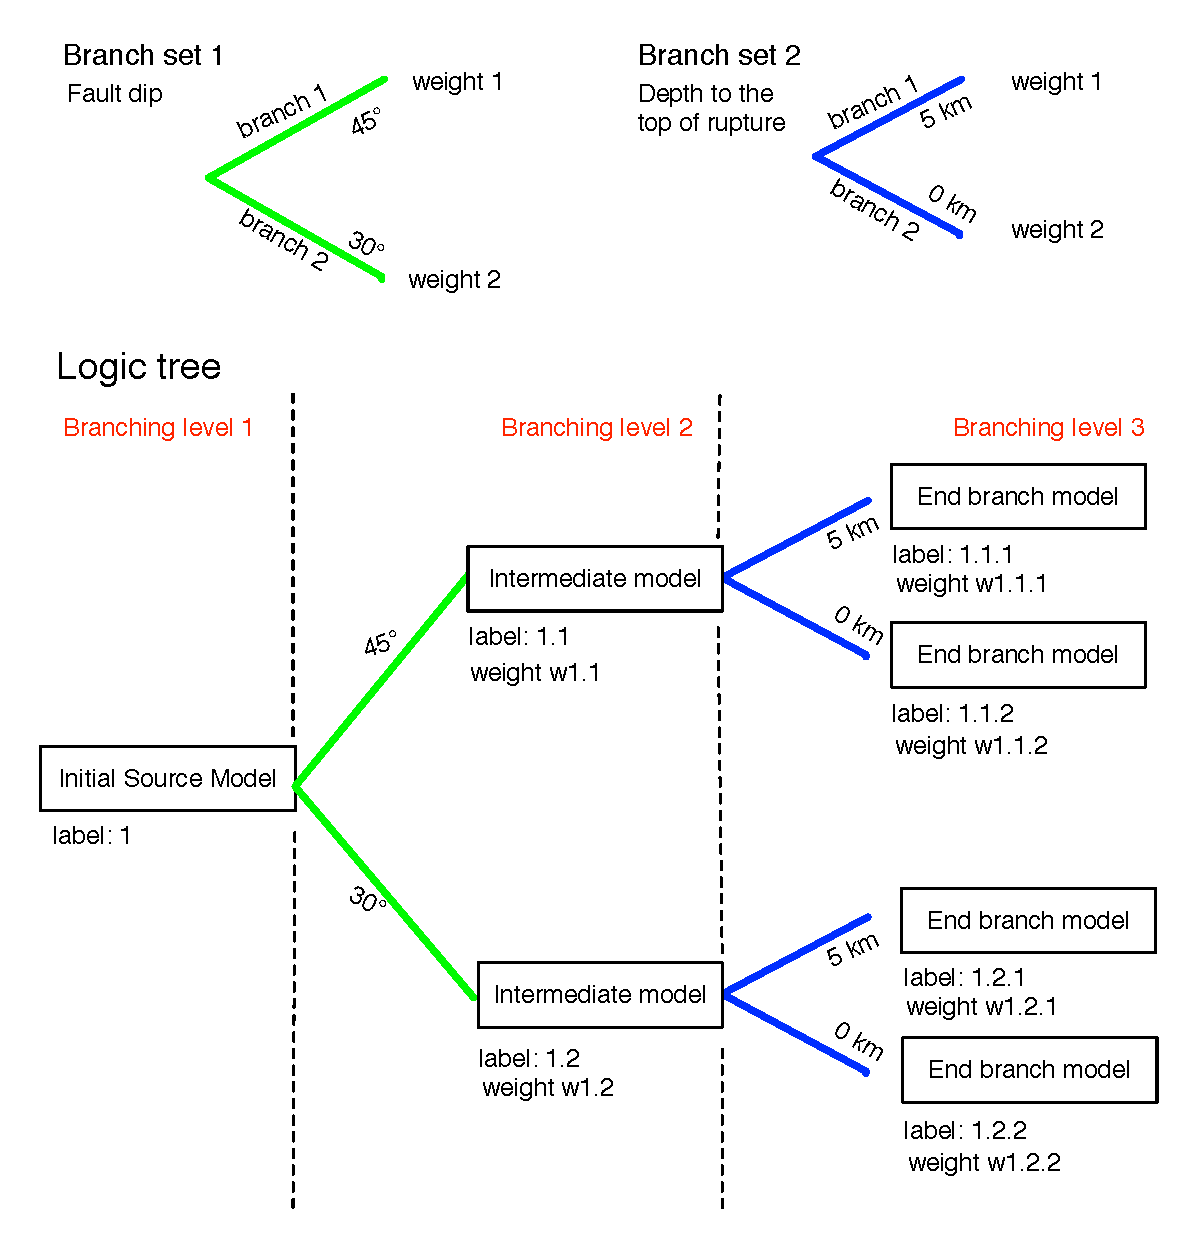
\includegraphics[width=15cm]{./Figures/Part_Hazard/logic_tree_schema.eps}
\caption{Example of a logic tree structure as defined in OpenQuake. The upper
part of the Figure depicts two branch sets.}
\label{fig:logic_tree_schema}
\end{figure}
% . . . . . . . . . . . . . . . . . . . . . . . . . . . . . . . . . . . < Figure
% ..............................................................................
%

This data model permits a very general definitions of logic tree 
structures. For instance, a non-symmetric logic tree can be easily 
created by placing multiple branch sets in the same branching level, each 
branch set being connected to a specific branch of a branch set defined in a
previous branching level. Figure \ref{fig:LogicTreeGeneralStructure}) shows a 
general example of a logic tree structure supported by OpenQuake logic tree 
data model. 

% ..............................................................................
% . . . . . . . . . . . . . . . . . . . . . . . . . . . . . . . . . . . > Figure
\begin{figure}
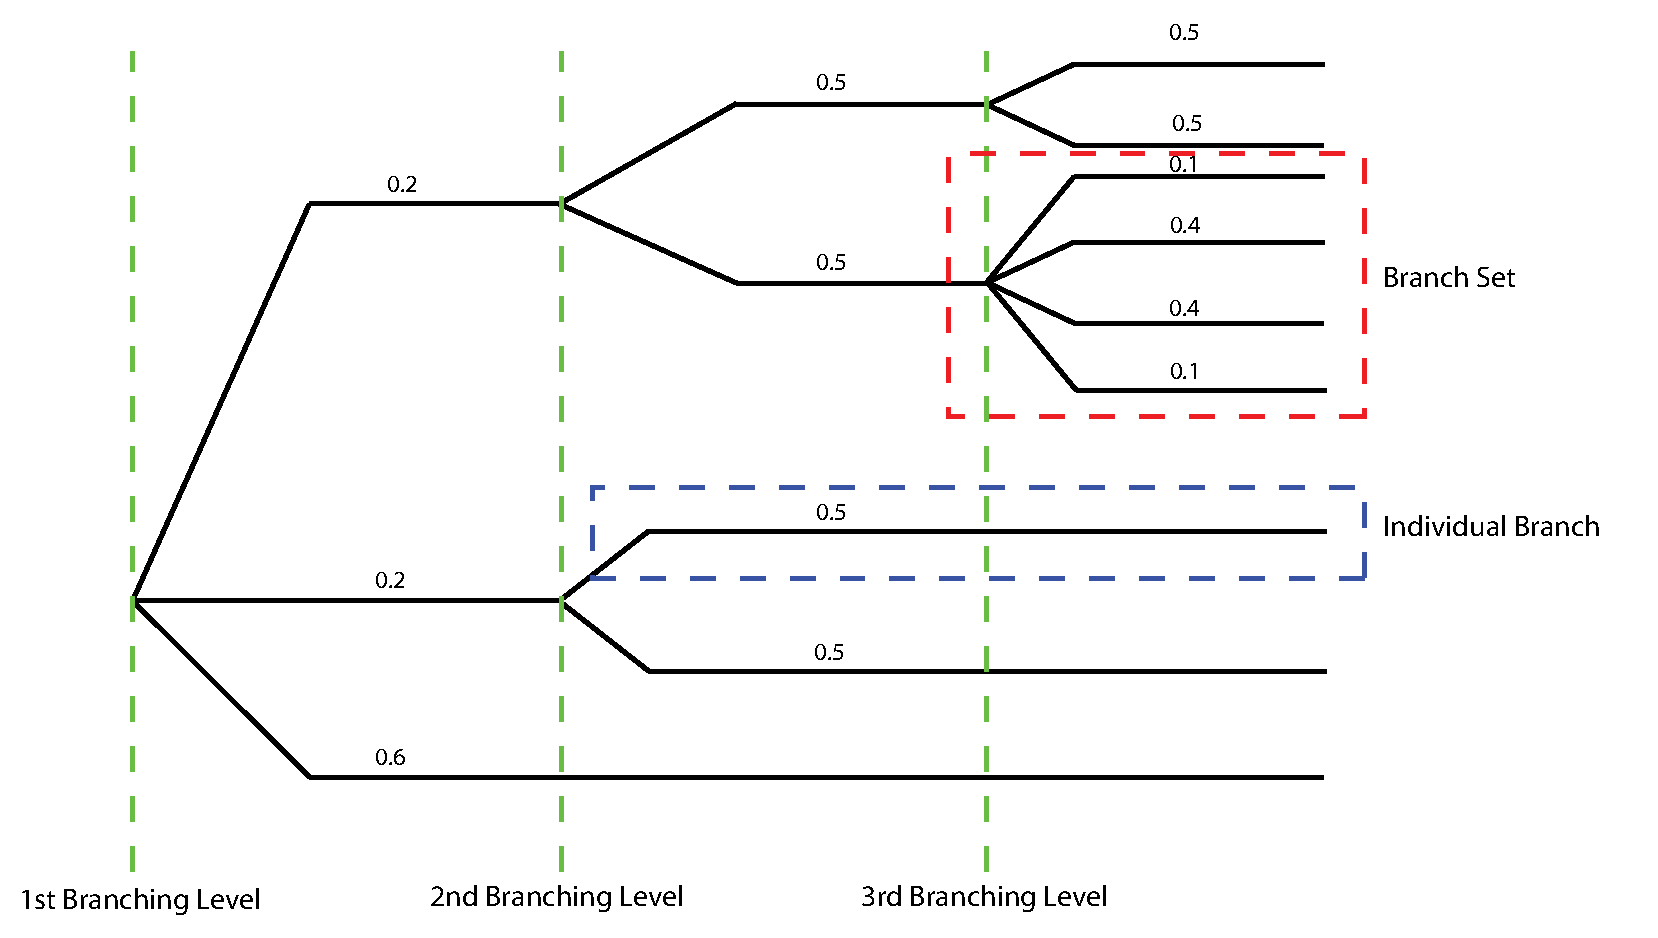
\includegraphics[width=15cm]{./Figures/Part_Hazard/LogicTreeGeneralStructure.eps}
\caption{Logic Tree data structure as defined in terms of individual branches, 
branch sets, and branching levels.}
\label{fig:LogicTreeGeneralStructure}
\end{figure}
% . . . . . . . . . . . . . . . . . . . . . . . . . . . . . . . . . . . < Figure
% ..............................................................................

We use this logic tree description to specify the structure of the Seismic 
Sources Logic Tree as well as for the Ground Motion Models Logic Tree. 
%  - - - - - - - - - - - - - - - - - - - - - - - - - - - - - - - - - - - - - - -
\subsection{Source Model Logic Tree}
\label{hazard:source_model_logic_tree}
%
In the current version of OpenQuake, a seismic sources model logic tree can be 
defined according to the following schema:
\begin{itemize}
\item The first branching level is assumed describing one or more "alternative" 
initial seismic source models.
\item Subsequent branching levels define source parameters uncertainties. 
Parameters uncertainties are applied independently to each seismic source 
in a source model. That is epistemic uncertainties are assumed uncorrelated 
between different seismic sources.
\item One branch set can be defined for branching level, thus assuming 
symmetric logic tree definition only.
\end{itemize}
%
The possibility of defining multiple source models in the first branching 
level responds to the need of modern PSHA of considering alternative source 
models (as derived by different expert opinions, for instance). 
%
Subsequent branching levels define the epistemic uncertainties that 
apply to parameters characterizing seismic sources. The  
epistemic uncertainties related to these parameters are implemented as 
\emph{rules}, that is as algorithms describing how this parameter has to be 
modified. 
%
The major advantage of using a rule-based approach is that a user does not 
need to a provide an input file containing a source model definition 
corresponding to a specific epistemic uncertainty, that is instead computed 
and applied on the fly to the initial model.
%
% ..............................................................................
% . . . . . . . . . . . . . . . . . . . . . . . . . . . . . . . . . . . > Figure
\begin{figure}
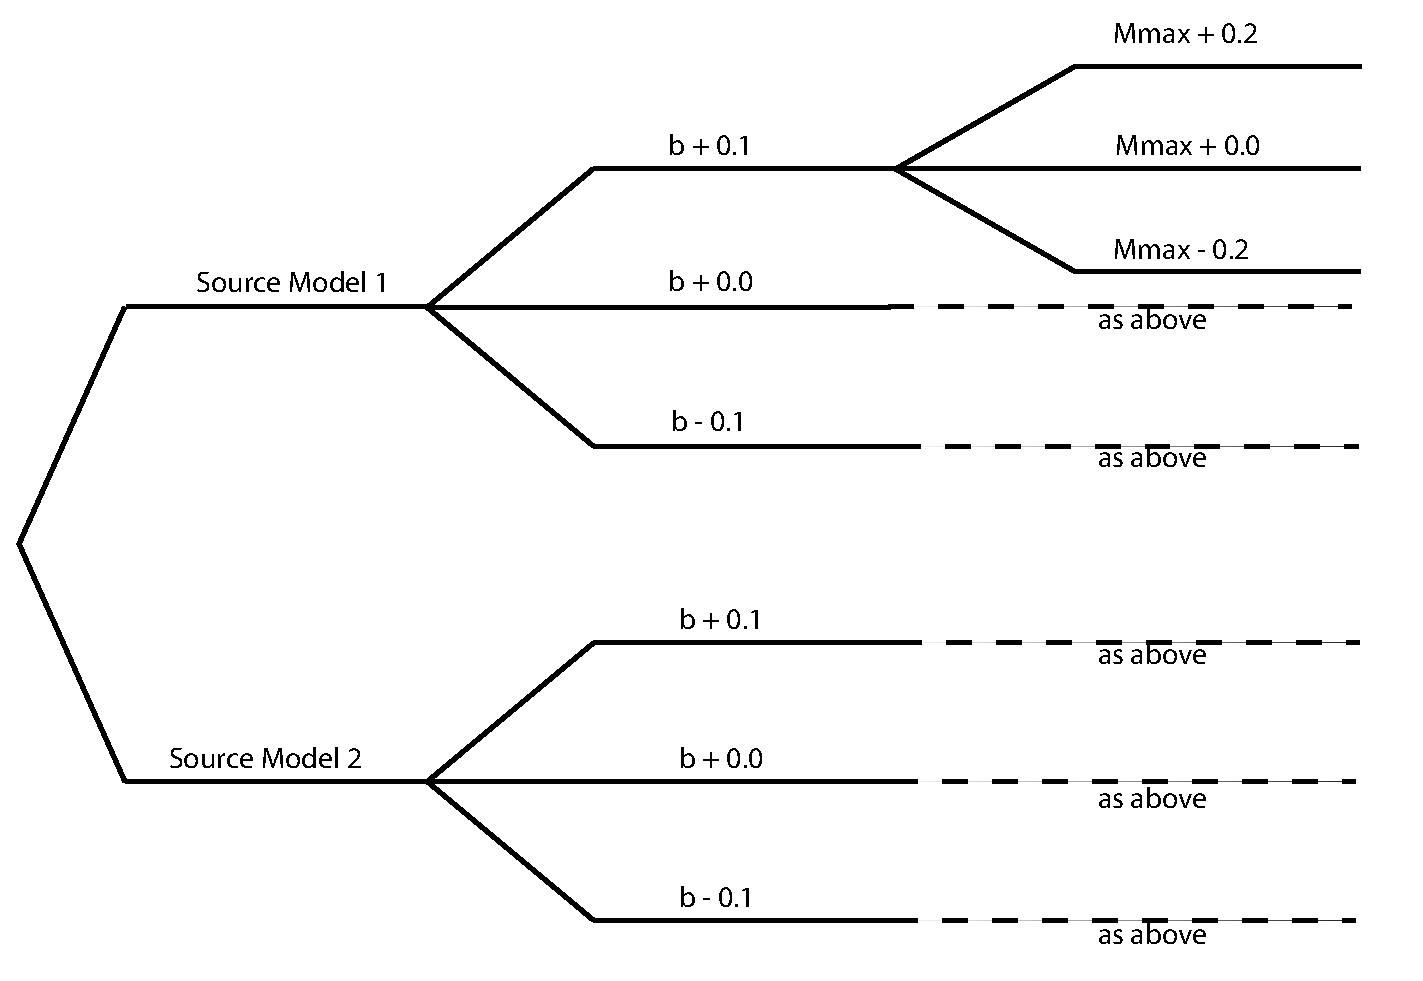
\includegraphics[width=15cm]{./Figures/Part_Hazard/SourceModelLogicTree.eps}
\caption{Example of Seismic Sources Logic Tree. The first branching level defines
two alternative source models (Source Model 1, Source Model 2). The second 
branching level defines uncertainties in b value (increment of 0.1, 0.0, -0.1).
The third branching level defines uncertainties in maximum magnitude 
(increments of 0.2, 0.0, -0.2).}
\label{fig:SourceModelLogicTree}
\end{figure}
% . . . . . . . . . . . . . . . . . . . . . . . . . . . . . . . . . . . < Figure
% ..............................................................................
%

The current version of OpenQuake offers two built-in rules:
\begin{itemize}
\item Gutenberg-Richter b value uncertainties. The user can specify a set 
of increments (positive or negative) that are added to Gutenberg-Richter 
b values. Conservation of total moment rate is assumed.
\item Gutenberg-Richter maximum magnitude uncertainties. The user can specify
a set of increments (positive or negative) that are added to Gutenberg-Richter 
maximum magnitude values. Conservation of total moment rate is assumed.
\end{itemize}
Figure \ref{fig:SourceModelLogicTree} depicts a source model logic tree that 
can be defined with the options currently present in OpenQuake.

The above mentioned rules are only a sample of possible source model epistemic 
uncertainties, and future versions of OpenQuake will provide a broader spectrum
of built-in epistemic uncertainties. Currently, rules are applied to all 
sources. Option to apply rules only to specific sources will be also supported 
in the future.
%  - - - - - - - - - - - - - - - - - - - - - - - - - - - - - - - - - - - - - - -
\subsection{GMPE Logic Tree}
\label{hazard:gmpe_logic_tree}
The GMPE Logic Tree allows a user to consider multiple ground motion prediction
equations in the hazard modeling. Given that GMPEs are often, or can be, 
associated to specific tectonic region types, OpenQuake allows the definition 
of multiple GMPE logic trees, one for each tectonic region type considered in 
the source model. In the current version, a GMPE logic tree can have only one 
branching level, containing only one branch set, where each individual branch 
is associated to a specific GMPE. With the current setting, epistemic 
uncertainties coming from different models can be taken into account, but 
epistemic uncertainties inside each model cannot be captured.
Figure \ref{fig:GMPELogicTree} schematically shows GMPE logic trees that can 
be currently defined in OpenQuake.
% ..............................................................................
% . . . . . . . . . . . . . . . . . . . . . . . . . . . . . . . . . . . > Figure 
\renewcommand{\psedge}{\ncdiag[armA=0,angleB=180,armB=1cm]}
\begin{figure}
\hfill \\
\textcolor{blue01}{\emph{Branch set definition}}: \dotfill
	GMPEs for active shallow crust regions \\
\textcolor{blue01}{\emph{Branch set uncertainty type}}: \dotfill
	Absolute values \\
\textcolor{blue01}{\emph{Applies to}}: \dotfill
	Active shallow crust sources   \\
\textcolor{blue01}{\emph{Correlated branches}}: \dotfill Yes \\
\hfill \\
\centering
	\begin{psTree}[treemode=R,levelsep=*2cm]
			{\Tr{ }}
		\begin{psTree}[treemode=R]{
			\Tr{\parbox[b]{4cm}{ GMPE$_1$ }}}%
		\end{psTree}%
		\begin{psTree}[treemode=R,treenodesize=1cm]{
			\Tr{\parbox[b]{4cm}{ GMPE$_2$ }}}%
		\end{psTree}%
		\begin{psTree}[treemode=R]{
			\Tr{\parbox[b]{4cm}{ GMPE$_3$ }}}%
		\end{psTree}%
	\end{psTree}%
\hfill \\
\hfill \\
\hfill \\
\textcolor{blue01}{\emph{Branch set definition}}: \dotfill
	GMPEs for subduction interface \\
\textcolor{blue01}{\emph{Branch set uncertainty type}}: \dotfill
	Absolute values \\
\textcolor{blue01}{\emph{Applies to}}: \dotfill
	Subduction interface sources \\
\textcolor{blue01}{\emph{Correlated branches}}: \dotfill Yes \\
\hfill \\
\centering
	\begin{psTree}[treemode=R,levelsep=*2cm]
			{\Tr{ }}
		\begin{psTree}[treemode=R]{
			\Tr{\parbox[b]{4cm}{ GMPE$_4$ }}}%
		\end{psTree}%
		\begin{psTree}[treemode=R,treenodesize=1cm]{
			\Tr{\parbox[b]{4cm}{ GMPE$_5$ }}}%
		\end{psTree}%
	\end{psTree}%
	
\hfill \\

\caption{Examples of GMPE Logic Trees. One for active shallow crust (considering
three GMPEs) and one for subduction interface (considering two GMPEs).}
\label{fig:GMPELogicTree}
\end{figure}

% . . . . . . . . . . . . . . . . . . . . . . . . . . . . . . . . . . . < Figure
% ..............................................................................